% Chapter Template

\chapter{Model Transformation} % Main chapter title

\label{Chapte3} % Change X to a consecutive number; for referencing this
% chapter elsewhere, use \ref{ChapterX}

\lhead{Chapter 3. \emph{Model Transformation}} % Change X to a consecutive 
% number; this is for the header on each page - perhaps a shortened title

In this chapter we will describe what model transformations is and also write
about the different types of model transformation. 
%----------------------------------------------------------------------------------------
%	SECTION 1
%----------------------------------------------------------------------------------------

\section{What is model transformation?}

Transformation is a fundamental theme in computer science and software
engineering. Whenever a computer starts up, transformation of computer systems
and computer programs happens frequently. Take a compiler for instance, it plays
a vital part of a computers internal infrastructure. A compiler is a computer
program that translates source code written in a high-level programming
language into lower level language, such as an assembly language or machine
code. This means that a computer program written in a general-purpose
programming language, such as Java or C++ would be useless without a compiler,
since the computer's central processing unit (CPU) depends on machine code to be
able to execute a set of instructions. But also computation of primitive data
values and performing operations on data structures such as lists and arrays can
also be viewed as data transformations. When a programming language provides a way
to type these data values or data structures, a compiler or interpreter can
apply operations to the data accordingly to the type. But when we talk about
data representing software artifacts such as a data schema, programs or models,
then transformation approaches 

%-----------------------------------
%	SUBSECTION 1
%-----------------------------------
\subsection{Basic concepts of model transformation}

The very basic concept of model transformations is to translate one model to
another model. This model translation can either be achieved through an
endogenous or an exogenous model transformation. For an endogenous model
transformation we take a source model expressed in a modelling language and
produce a target model expressed in the same language. While an exogenous model
transformation start with a source model expressed in one modelling language and
translate this into a target model expressed in another modelling language. It
is essential that these models remain consistent, and therefore both the source
and target model have to conform to their corresponding metamodel.
Figure~\ref{fig:BasicTransformation} is a representation of the basic concepts
for a model transformation. The two concepts, transformation language and
transformation engine are provided by some model transformation environment.
The transformation language use metadata that are defined in the source and
target metamodel to create an executable environment for the transformation
engine. 

It is essential that these models are consistent. This is
obtained through the use of metamodels.
A model transformation can produce two different kind of output models. The
first one is code generation, often referred to Model to Text(M2T)
transformation, and it takes one model and produces implementation code. This
is convenient if for example a software engineer wants to produce source code

\begin{figure}[H]
  \centering
    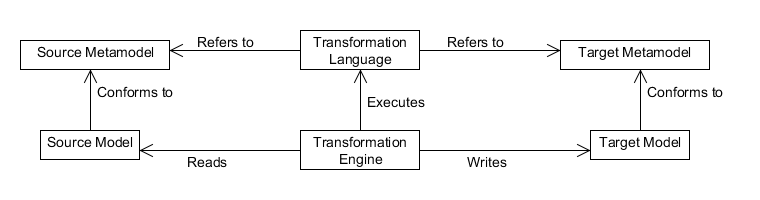
\includegraphics[scale=0.5]{./Figures/BasicTransformation.png}
    \rule{35em}{0.5pt}
  \caption[Basic Model Transformation]
  				{The basic concepts behind a model
  transformation.}
  \label{fig:BasicTransformation}
\end{figure}

\section{Model Transformation in MDE}

%-----------------------------------
%	SUBSECTION 2
%-----------------------------------

\section{Classification of a model transformation}

In March 2006 Krzysztof Czarnecki and Simon Helsen did a domain analysis to
existing model transformation approaches\cite{Czarnecki2006}. A domain analysis represents
information on software system that share a common set of features for a given
domain\cite{FODA,Prieto-Diaz1990}, in this case the domain is model
transformations. This section is based on the ideas and result from Czarnecki
and Helsen's report. In their paper they presents a feature diagram that
provides a terminology and representation of the design choices for model
transformation approaches. This feature diagram does not only present model to
model approaches, but also consider the design choices for model to text
approaches. For the purpose of this thesis we will only address the model to
model approaches in Czarnecki and Helsen's survey on model transformations.
However it is important to address that at top level, we can divide model
transformations into to categories, namely model to text and model to model
transformations. The major difference between these categories are that model to
model transformations generate a target model as an instance of the targets
metamodel. While the target of a model to text transformation are string
sequences. Model to text transformation are also often referred to as model to
code transformation since a collection of strings can be source code that
corresponds to some programming language. 

\begin{figure}[H]
  \centering
    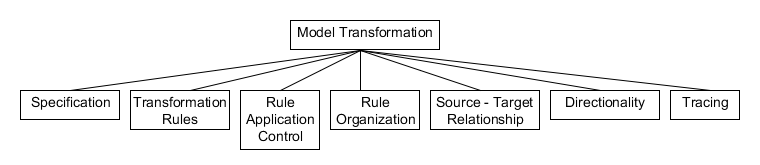
\includegraphics[scale=0.6]{./Figures/Model_Transformation_Survey.png}
    \rule{35em}{0.5pt}
  \caption[Domain Analysis of Model Transformations]
  				{A domain analysis of model transformations\cite{Czarnecki2006}.}
  \label{fig:Model_Transformation_Survey}
\end{figure}

Figure~\ref{fig:Model_Transformation_Survey} shows the feature diagram at top
level of a model transformation, where each subnode represents a major aspect
of model transformations. 

\subsection{Specification}

\subsection{Transformation Rules}

For a model transformation to be able to translate a model to another model it
needs a set of guidelines on how this should be done. Therefore a model
transformation has a set of transformation rules that specifies how a target
model should be produced. An obvious example of such rules are the rewrite
rules. A rewrite rule provides a left hand side (LHS) and a right hand side
(RHS) and both sides represents some user created patterns that are considered
when a transformation engine executes their corresponding transformation rules.
But a function that implements some transformation steps can also be seen as a
transformation rule. For example in ATL Transformation Language (ATL) \cite{ATL}
a transformation rule is implemented as a function, that consists of various
steps on how this transformation rule should be applied. 

Every transformation rule has a metamodel attached. A metamodel is referred
to as a domain in Czarnecki and Helsen's survey\cite{Czarnecki2006}. This
is to make the term metamodel a more general term since some transformation
languages take other approaches to how these metamodels are created. The
Attributed Graph Grammar System\cite{AGG} (AGG) for example, uses a common type
graph for both source and target model that contains all possible elements that
are available to create transformation rules. Therefore its better to use the
term domain when we are discussing transformation rules in general. These
domains are usually represented as a source and a target domain for a
transformation rule. However a transformation rule is not necessary bound to
only a source and a target domain, but can also have several other domains to
its disposal. 

These domains for a transformation rule are expressed in a language that
describes the possible structures for a model for that domain. When we operate
on models expressed in the context of MDA, then the language of the domain has
the form of a metamodel expressed in MOF\cite{MOF}.


\subsection{Rule Application Control}

The transformation rule has to 

\subsection{Rule Organization}

\subsection{Source - Target Relationship}

\subsection{Directionality}

\subsection{Tracing}


%----------------------------------------------------------------------------------------
%	SECTION 2
%----------------------------------------------------------------------------------------

\section{Graph Transformation} 

One approach to model transformations is by graph transformations,
also referred to as graph rewriting. Graph rewriting can be implemented with
an algebraic approach, which is based on Category Theory. Before we go into
detail about graph transformation, we should quickly describe the concepts of
Category Theory\cite{Herrlich1973,Barr1990}. Category theory can be used to
formalize mathematical or software theory's at a high level of abstraction. In
2006 Steve Awodey published a second edition of the book, Category Theory,
where he stated,

``Just as group theory is the abstraction of the idea of a system of
permutations of a set or symmetries of a geometric object, category theory
arises from the idea of a system of functions among some
objects\cite{Awodey2006}.''

\begin{figure}[H]
	\centering
	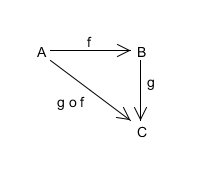
\includegraphics[scale=0.7]{./Figures/categoryTheory.png}
	\caption[Category Theory]
	{Collection of objects A,B and C.}
	\label{fig:categoryTheory}
\end{figure}

Category Theory can be used as a supplement to explain the theoretical aspects
behind a problem or solution. A category consists of a collections of
objects and functions. In figure~\ref{fig:categoryTheory} we have a collection
of objects A, B, C and arrows f, g, g $\circ$ f. The figure describe that
there is a connection between the two objects A and B. This connection
indicates that there are some association between two objects. For this case
this means that function f is defined in A and the values of this function are
in B. When the objects represents graphs, then these connections between objects
are often referred to as morphisms between graphs or graph morphisms. Morphisms
are pair of maps which commute with source and target\cite{Brown2008}.
Figure~\ref{fig:categoryTheory} has three sets of graph morphisms, f : A
$\longrightarrow$ B, g : B $\longrightarrow$ C and g $\circ$ f : A
$\longrightarrow$ C. The last set of graph morphisms, g $\circ$ f indicates that
there is a composite function between A and C. This basically means that if
C is a function g of B and B is a function f of A, then C is the result of a
function between C and A. 

For the purpose of this thesis the collection of objects represents graphs the
arrows represents morphisms. A graph contains a collection of nodes and edges.
A graph is undirected when there is no distinction between two nodes associated
with an edge or it is a directed graph if an edge has a direction between two
nodes. This means that each node is represented as a source and a target node
for an edge. A directed graph L can be defined by L = \{
N\textsubscript{L}, E\textsubscript{L}, source\textsubscript{L},
target\textsubscript{L} \}. N\textsubscript{L} represents the collection of
nodes and E\textsubscript{L} represents the collection of edges that are
included for the directed graph. The third and forth elements,
source\textsubscript{L} and target\textsubscript{L}, are functions that
retrieves the source and target node for an edge. This collection of nodes and
edges in a graph L can result in an excact match in another graph G. The
morphism between these two graphs are called homomorphism.

\subsubsection*{Graph Homomorphism}

When a graph that has a mapping of nodes and edges in another graph, then there
is a graph homomorphism between these two graphs.

\begin{figure}[H]
	\centering
	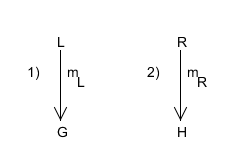
\includegraphics[scale=0.7]{./Figures/GraphHomomorphism.png}
	\caption[Basic concepts of graph homomorphism]
	{Two sets of graph homomorphism of graph L in G and R in H}
	\label{fig:graphHomomorphism}
\end{figure}

Figure~\ref{fig:graphHomomorphism} has two graph homomorphisms
\mbox{L$\xrightarrow{m\textsubscript{L}}$G} and 
\mbox{R$\xrightarrow{m\textsubscript{R}}$H}. Now if we consider the first
example, if there is to be a valid graph homomorphism between graph L and G,
then the collection of nodes and edges in L has to be mapped to nodes and edges
in G. If both graphs L and G are directed graphs we can safely assume that the
definition of graph L in the last paragraph is also true for graph G =\{
N\textsubscript{G}, E\textsubscript{G}, source\textsubscript{G},
target\textsubscript{G} \}. For a graph homomorphism m\textsubscript{L} from the
graph L to the graph G, \mbox{L$\xrightarrow{m\textsubscript{L}}$G}, there is a
mapping m\textsubscript{L} : N\textsubscript{L} $\longrightarrow$
N\textsubscript{G} from the set of nodes in graph L to the set of nodes in
graph G and a mapping mapping m\textsubscript{L} : E\textsubscript{L}
$\longrightarrow$E \textsubscript{G} from the set of edges in graph L to the
set of edges in graph G that preserve both source and target nodes. This means
that there is a mapping from a source node in G that is equal to a source node
in L and a target node in G is equal to a target node in L. 

\subsection{The Algebraic Approach}
This approach are based on the concepts of composing graphs, modelled
by pushouts of graphs and graph morphisms. This pushout approach comes in
different variants, and we will look at two of these, namely the
double-pushout (DPO) approach and the single pushout (SPO)
approach\cite{Loewe1997,Ehrig1997}.

Historically, the first of the algebraic approaches to graph
transformations, the double-pushout, was first introduced at the Technical
University of Berlin in the early seventies by H. Ehrig, M. Pfender and H.J.
Schneider\cite{INSPEC:606170}. They tried to generalize Chromsky grammars from
strings to graphs. This allowed to define a graph rewriting step by the use of
two gluing constructions. And by applying a graph rewriting step for the
double-pushout approach is a pair of morphisms in the category of graphs where
the arrows represents total graph morphisms, \mbox{L $\longleftarrow$
\ K $\longrightarrow$ R}. This is true for each application rule in a graph
transformation for the double-pushout approach. Where the graph K represents the
common part and the two morphisms \mbox{L $\longleftarrow$ \ K} and \mbox{K
$\longrightarrow$ R} use the algebraic construction, pushout to apply an
application rule for a rewriting step. Hence the name double pushout and the use
of two rewriting conditions.

\subsection{Productions}
For a transformation language to be able to execute graph
transformations a set of application rules needs to be defined. Through these
rules, a transformation interpreter can act accordingly. These rules are often
referred to as Productions. For graph transformations, there can be an arbitrary
number of rules. Its truly up to the users how they want to translate a
language and how many rules that is needed to acquire this. Each rule consists
of a left hand side (LHS) and a right hand side (RHS), also often referred to as
pattern graph and replacement graph. The pattern graph represents a subgraph of
the model that is going to be translated, namely the host graph. For these
productions to execute, there has to be some control mechanism, namely the
transformation unit.

\subsection{Transformation Units}
In graph transformation, there has to be a control mechanism that
administrates these productions. These control mechanisms are also called
transformation units. These units controls the order that the transformation
rules are executed. The most basic transformation unit is a rule itself which
corresponds to a single application of that rule. But in most cases, a
transformation unit will have to control several rule applications. 

\subsection{A Direct Derivation}
The basic idea for graph transformation for both the double-pushout
approach and the single pushout approach is to apply an application rule
\mbox{r: L $\longrightarrow$ R}. Where the rule represents a single rewriting
step for graph transformations and L represents the left hand side of the rule and R
represents the right hand side of the rule.

\begin{figure}[H]
	\centering
	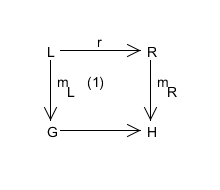
\includegraphics[scale=0.7]{./Figures/Single_Pushout.png}
	\caption[Idea of graph transformation]
	{The basic idea for graph transformation by applying a rule r.}
	\label{fig:GraphTransformationGeneral}
\end{figure}

For a production rule r, \mbox{G$\xrightarrow{r,m}$G'} indicates a direct
derivation to a derived graph G'. In
figure~\ref{fig:GraphTransformationGeneral}, the graph G' is created by
applying a single pushout for a transformatin rule r. If there is a match m of
nodes and arrows for a subgraph L in a host graph G, then this indicates a
graph homomorphism, mapping elements from the subgraph to the host graph in
such a way that the graphical structure in G is preserved. For each rule r,
there are some algebraic approaches to how we can achieve G'. At this moment
there are four approaches, the double-pushout approach (DPO) \cite{Loewe1997}, the
single-pushout approach (SPO) \cite{Ehrig1997}, the sesqui-pushout and the
pullback approach. Where the two most common approaches used in graph
transformation tools are the DPO and the SPO approach. There is one major
aspect that separate these two approaches, and that is that the DPO approach
has an application condition.

\begin{figure}[H]
	\centering
	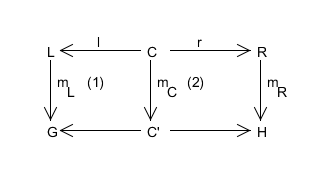
\includegraphics[scale=0.7]{./Figures/Double_Pushout.png}
	\caption[The Double Pushout approach]
	{Principles behind the double pushout approach.}
	\label{fig:DPO}
\end{figure}

\noindent This application condition, named the gluing condition\cite{Loewe1997}
consists of two parts. Namely the dangling condition and identification
condition. From figure~\ref{fig:DPO}, the dangling condition requires that if
the transformation rule p specifies the deletion of a node in G, then it must also
specify the deletion of all incoming and outgoing edges of this node in G. By
applying this condition, we can be sure that there are no dangling edges after
deleting a node in G. The identification condition requires that every element
of G that should be deleted by applying a transformation rule p is only present
once in L for each transformation rule p. 

A single transformation rule p in the DPO approach is given by a pair of graph
homomorphisms from a common graph C. This common graph C is formed by taking
elements that are present in both L (LHS) and R (LHS) of a transformation rule
p. The graph G' are created from the graph G, by deleting all elements that is
matched from the pattern graph L, but none in C. To avoid dangling edges,
the gluing condition must be satisfied before deleting these elements. This is
the first part (1) of the DPO approach, namely the deletion of elements. The
second part (2) is insertion of elements. From here we create a graph H off all
nodes and arrows from the replacement graph R that is not presented in the
common graph C. The DPO approach has the possibility to preserve elements from
translating from the pattern graph L and the replacement graph R with the help
of a common graph C.

For the SPO approach on the other hand, deletion has priority over preservation.
Figure~\ref{fig:GraphTransformationGeneral} is a representation of the practices
of the SPO approach. Where nodes that are present in the pattern graph L but not
the replacement graph R are deleted. And the incoming and outgoing edges of the
deleted nodes that are not present in the replacement graph R is deleted.

Now that we have explained some aspects of Graph transformations, we can
describe the three different tools, where both AGG and Henshin is build around
the concepts of graph transformations explained in this section. 

\begin{figure}[H]
	\centering
	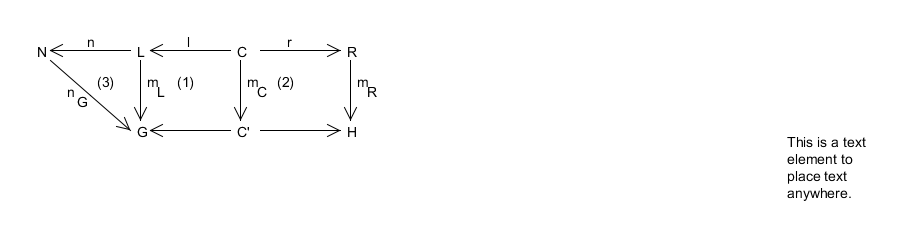
\includegraphics[scale=0.7]{./Figures/Double_Pushout_NAC.png}
	\caption[The Double Pushout approach with NAC]
	{Double pushout approach with negative application condition.}
	\label{fig:DPO_NAC}
\end{figure}

\begin{figure}[H]
	\centering
	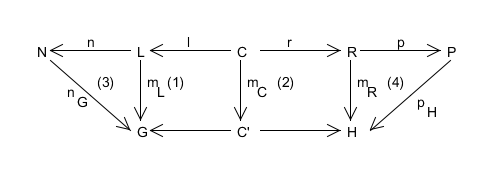
\includegraphics[scale=0.7]{./Figures/Double_Pushout_PAC.png}
	\caption[The Double Pushout approach with PAC]
	{Double pushout approach with positive application condition.}
	\label{fig:DPO_NAC}
\end{figure}

\section{Textual Model Transformation}



